% !TeX encoding = UTF-8
\documentclass[10pt,twocolumn]{article}
% This project deliberately uses only standard Overleaf packages.
\usepackage[margin=0.78in]{geometry}
\usepackage{graphicx,amsmath,amssymb,booktabs,multirow,array,xcolor,url,enumitem,microtype}
% Keeps pdfLaTeX compatible with TeX installations lacking scalable font maps.
\microtypesetup{expansion=false}
\usepackage{natbib}
\usepackage{tikz,pgfplots}
\usetikzlibrary{arrows.meta,positioning,calc,shapes.geometric,decorations.pathreplacing}
\pgfplotsset{compat=1.18}
\definecolor{paperblue}{RGB}{35,92,145}
\definecolor{papergreen}{RGB}{51,122,88}
\definecolor{paperorange}{RGB}{207,119,42}
\definecolor{paperred}{RGB}{178,59,49}
\usepackage[colorlinks=true,linkcolor=paperblue,citecolor=paperblue,urlcolor=paperblue]{hyperref}
\usepackage{listings}
\usepackage{placeins,needspace}

% Data-driven schematic figures. Values trace to report/evidence_summary.md.
\newcommand{\PipelineFigure}{%
\begin{figure*}[t]
\centering
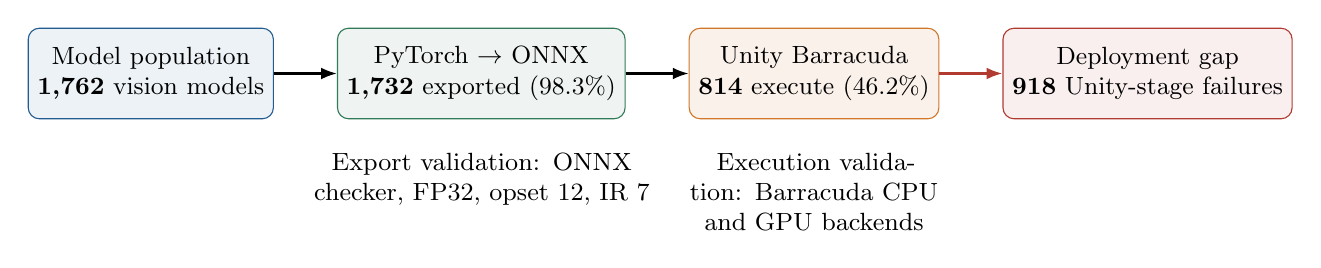
\begin{tikzpicture}[font=\small,node distance=8mm,every node/.style={align=center}]
\node[draw=paperblue,fill=paperblue!8,rounded corners,minimum width=3.0cm,minimum height=1.15cm] (a) {Model population\\\textbf{1,762} vision models};
\node[draw=papergreen,fill=papergreen!8,rounded corners,minimum width=3.0cm,minimum height=1.15cm,right=of a] (b) {PyTorch $\rightarrow$ ONNX\\\textbf{1,732} exported (98.3\%)};
\node[draw=paperorange,fill=paperorange!10,rounded corners,minimum width=3.0cm,minimum height=1.15cm,right=of b] (c) {Unity Barracuda\\\textbf{814} execute (46.2\%)};
\node[draw=paperred,fill=paperred!8,rounded corners,minimum width=2.5cm,minimum height=1.15cm,right=of c] (d) {Deployment gap\\\textbf{918} Unity-stage failures};
\draw[-{Latex[length=2mm]},thick] (a)--(b); \draw[-{Latex[length=2mm]},thick] (b)--(c); \draw[-{Latex[length=2mm]},thick,paperred] (c)--(d);
\node[below=3mm of b,text width=5.2cm] {Export validation: ONNX checker, FP32, opset 12, IR 7};
\node[below=3mm of c,text width=4.2cm] {Execution validation: Barracuda CPU and GPU backends};
\end{tikzpicture}
\caption{The measured deployment pipeline. The dominant observed attrition occurs after successful ONNX export, at the Unity Barracuda stage. Execution success denotes a valid benchmark result, not numerical output equivalence.}
\label{fig:pipeline}
\end{figure*}%
}

\newcommand{\CompatibilityFigure}{%
\begin{figure}[t]\centering
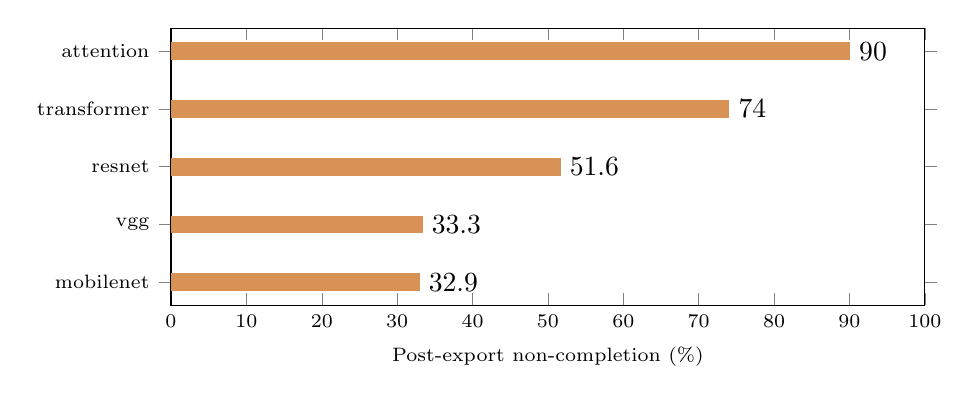
\begin{tikzpicture}\begin{axis}[xbar,width=.92\columnwidth,height=5.1cm,xmin=0,xmax=100,xlabel={Post-export non-completion (\%)},ytick=data,yticklabels={MobileNet-like (76),VGG-like (18),ResNet-like (630),Transformer-like (146),Attention (10)},bar width=6pt,nodes near coords,nodes near coords align={horizontal},tick label style={font=\scriptsize},label style={font=\scriptsize},symbolic y coords={mobilenet,vgg,resnet,transformer,attention}]
\addplot[fill=paperorange!80,draw=paperorange!80] coordinates {(32.9,mobilenet) (33.3,vgg) (51.6,resnet) (74.0,transformer) (90.0,attention)};
\end{axis}\end{tikzpicture}
\caption{Post-export non-completion by architecture flag. Denominators are export-successful models carrying each non-exclusive flag; the attention estimate is based on only 10 models. These are associations, not causal diagnoses.}
\label{fig:compatibility}\end{figure}%
}

\newcommand{\ReproducibilityFigure}{%
\begin{figure}[t]\centering
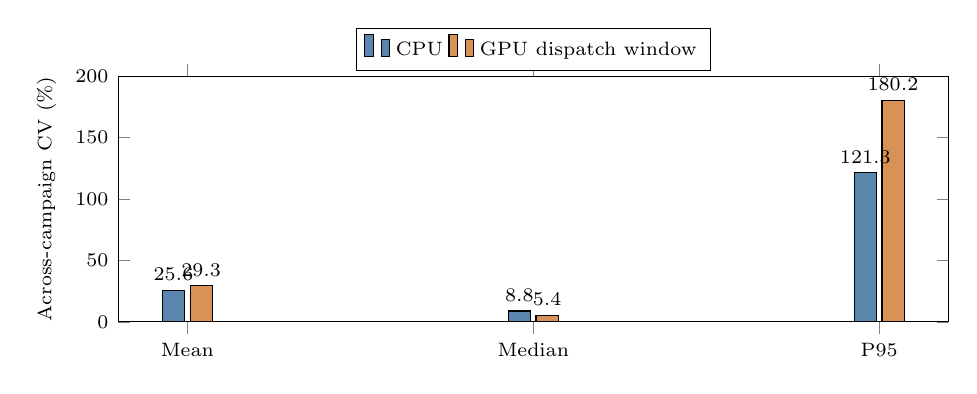
\begin{tikzpicture}\begin{axis}[ybar,width=\columnwidth,height=4.7cm,ymin=0,ymax=200,ylabel={Across-campaign CV (\%)},symbolic x coords={Mean,Median,P95},xtick=data,bar width=8pt,legend style={font=\scriptsize,at={(0.5,1.02)},anchor=south,legend columns=2},tick label style={font=\scriptsize},label style={font=\scriptsize},nodes near coords,every node near coord/.append style={font=\scriptsize}]
\addplot[fill=paperblue!75] coordinates {(Mean,25.6) (Median,8.8) (P95,121.3)};
\addplot[fill=paperorange!80] coordinates {(Mean,29.3) (Median,5.4) (P95,180.2)};
\legend{CPU,GPU dispatch window}\end{axis}\end{tikzpicture}
\caption{Per-model timing-CV summaries across six RTX~4090 campaigns. Low medians coexist with very high 95th percentiles; aggregate completion stability does not imply uniform timing stability.}
\label{fig:reproducibility}\end{figure}%
}

\newcommand{\TimingFigure}{%
\begin{figure*}[t]\centering
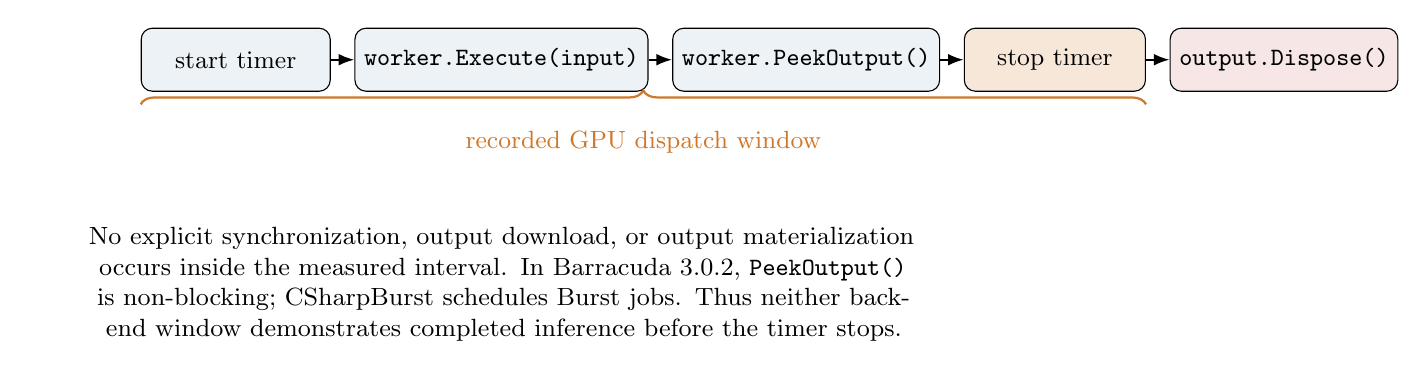
\begin{tikzpicture}[font=\small,node distance=3mm]
\node[draw,rounded corners,fill=paperblue!8,minimum width=2.4cm,minimum height=8mm] (start) {start timer};
\node[draw,rounded corners,fill=paperblue!8,minimum width=2.8cm,minimum height=8mm,right=of start] (execute) {\texttt{worker.Execute(input)}};
\node[draw,rounded corners,fill=paperblue!8,minimum width=2.8cm,minimum height=8mm,right=of execute] (peek) {\texttt{worker.PeekOutput()}};
\node[draw,rounded corners,fill=paperorange!18,minimum width=2.3cm,minimum height=8mm,right=of peek] (stop) {stop timer};
\node[draw,rounded corners,fill=paperred!12,minimum width=2.7cm,minimum height=8mm,right=of stop] (dispose) {\texttt{output.Dispose()}};
\draw[-{Latex[length=2mm]},thick] (start)--(execute); \draw[-{Latex[length=2mm]},thick] (execute)--(peek); \draw[-{Latex[length=2mm]},thick] (peek)--(stop); \draw[-{Latex[length=2mm]},thick] (stop)--(dispose);
\draw[decorate,decoration={brace,amplitude=5pt},paperorange,thick] ($(start.south west)+(0,-.16)$) -- ($(stop.south east)+(0,-.16)$) node[midway,below=6pt,text=paperorange] {recorded GPU dispatch window};
\node[below=16mm of execute,align=center,text width=11.8cm] {No explicit synchronization, output download, or output materialization occurs inside the measured interval. In Barracuda 3.0.2, \texttt{PeekOutput()} is non-blocking; CSharpBurst schedules Burst jobs. Thus neither backend window demonstrates completed inference before the timer stops.};
\end{tikzpicture}
\caption{Timing-semantics audit of the Unity benchmark implementation. The placement of the timer bounds is central to interpreting every backend result in this article.}
\label{fig:timing-semantics}\end{figure*}%
}

\newcommand{\CorrelationFigure}{%
\begin{figure}[t]\centering
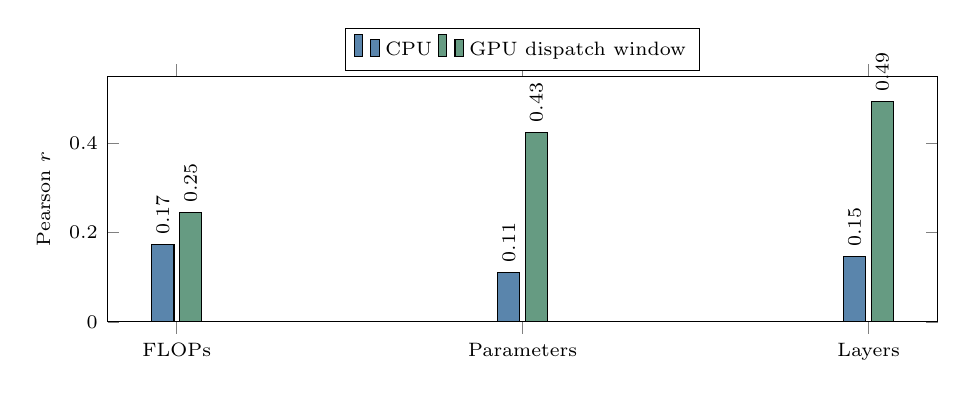
\begin{tikzpicture}\begin{axis}[ybar,width=\columnwidth,height=4.7cm,ymin=0,ymax=.55,ylabel={Pearson $r$},symbolic x coords={FLOPs,Parameters,Layers},xtick=data,bar width=8pt,legend style={font=\scriptsize,at={(0.5,1.02)},anchor=south,legend columns=2},tick label style={font=\scriptsize},label style={font=\scriptsize},nodes near coords,every node near coord/.append style={font=\scriptsize,rotate=90,anchor=west}]
\addplot[fill=paperblue!75] coordinates {(FLOPs,.173) (Parameters,.111) (Layers,.146)};
\addplot[fill=papergreen!75] coordinates {(FLOPs,.245) (Parameters,.425) (Layers,.493)};
\legend{CPU,GPU dispatch window}\end{axis}\end{tikzpicture}
\caption{Raw Pearson associations for 811 models with metadata. Conventional complexity descriptors are at most moderate correlates of the recorded measurements.}
\label{fig:correlations}\end{figure}%
}


\begin{document}
\title{The Deployment Gap: Compatibility, Reproducibility, and Runtime Behavior\\of 1,762 Vision Models in the PyTorch--ONNX--Unity Barracuda Pipeline}
\author{Syed Ali Haider\thanks{Correspondence: \texttt{\scriptsize syed.haider@stud-mail.uni-wuerzburg.de}} \quad Radu Timofte \quad Dmitry Ignatov\\
\small Computer Vision Lab, CAIDAS \& IFI, University of W\"urzburg, Germany}
\date{}
\maketitle

\PipelineFigure

%% ============================================================
%% 1. ABSTRACT
%% ============================================================
\begin{abstract}
Deploying a vision model inside a game engine is fundamentally a deployment problem, not merely an inference-speed problem.
We study 1,762 pretrained vision architectures transferred through the PyTorch $\rightarrow$ ONNX $\rightarrow$ Unity Barracuda pipeline and systematically evaluate six research questions spanning compatibility, reproducibility, runtime behavior, architecture--timing-window relationships, Unity-vs-standalone comparison, and VR deployment implications.
ONNX export succeeds for 1,732 models (98.3\%), yet only 814 models (46.2\%) complete a Unity Barracuda benchmark, revealing that the major deployment barrier occurs \emph{after} export.
Among export-successful models carrying each flag, post-export non-completion is 90.0\% for attention-flagged and 74.0\% for Transformer-like models, versus 32.9\% for MobileNet-like models; flags overlap and these are descriptive associations.
Six RTX~4090/Vulkan campaigns show stable aggregate completion counts (811--814) with 806 of 814 models present in all six campaigns, but per-model timing coefficients of variation exhibit a heavy tail (CPU CV p95 = 121.3\%; GPU dispatch-window CV p95 = 180.2\%), demonstrating that aggregate stability does not imply universal timing reproducibility.
We document that the Unity benchmark records a backend timing window around \texttt{worker.Execute}--\texttt{worker.PeekOutput} without forcing output materialization. In the vendored Barracuda~3.0.2 source, \texttt{PeekOutput()} is non-blocking and \texttt{CSharpBurst} schedules Burst jobs; therefore neither CPU nor GPU values are validated completed-inference latencies.
Software-emulated GPU execution via Mesa llvmpipe reverses the apparent CPU/GPU ordering, confirming that emulated benchmarks are unsuitable for hardware performance decisions.
Conventional complexity measures (FLOPs, parameter count, layer count) show weak-to-moderate Pearson correlations with recorded timings ($r \leq 0.49$), indicating that standalone complexity metrics are insufficient predictors of game-engine runtime behavior.
An observational Unity/workstation comparison on 814 matched models shows Spearman rank agreement of 0.753 (CPU) and 0.741 (GPU), but the comparison is protocol-mismatched and cannot establish a portable multiplicative overhead.
Our central conclusion is that successful standalone inference or ONNX export does not guarantee successful deployment in a game-engine inference runtime, and model selection for VR/XR must be validated in the actual deployment environment.
\end{abstract}

%% ============================================================
%% 2. INTRODUCTION
%% ============================================================
\section{Introduction}\label{sec:introduction}

Real-time XR applications---including virtual reality (VR), augmented reality (AR), and mixed reality (MR)---increasingly embed deep-learning vision models directly inside a game engine rather than in a standalone machine-learning runtime. Unity, one of the dominant engines for XR development, provides the Barracuda inference library for executing neural networks from ONNX~\cite{onnx2019} graphs at runtime. The deployment path from a trained PyTorch model to real-time Unity execution introduces at least three distinct questions that cannot be answered by a single FLOPs count or standalone benchmark:

\begin{enumerate}[nosep,leftmargin=*]
  \item \textbf{Can the model be exported?} PyTorch's ONNX exporter must successfully trace or script the model graph.
  \item \textbf{Can the target runtime execute the graph?} The ONNX importer in Unity Barracuda must support every operator, shape, and graph pattern.
  \item \textbf{Can execution meet the application's latency budget?} The runtime behavior of the executed model must be compatible with real-time frame deadlines.
\end{enumerate}

Treating FLOPs or a standalone PyTorch timing as an answer to all three is unsafe. A model that runs efficiently in PyTorch may fail to export, fail to import into Unity, crash at execution time, or produce timing behavior unrelated to its theoretical complexity. This paper examines that gap for a large, diverse collection of 1,762 vision architectures from the LEMUR/NN-Dataset ecosystem~\cite{ABrain.NN-Dataset, ABrain.LEMUR2}.

Our central research question is: \emph{How reliably do diverse vision architectures traverse the PyTorch--ONNX--Unity Barracuda pipeline, and what can the available measurements establish about runtime behavior, reproducibility, and VR deployment readiness?}

The study is organized around six research questions (Section~\ref{sec:rqs}) that span compatibility, reproducibility, runtime behavior, architecture--timing-window relationships, Unity-vs-standalone comparison, and practical VR deployment implications.

\paragraph{Contributions.}
Our contributions are deliberately scoped to the evidence available in the repository:
\begin{enumerate}[nosep,leftmargin=*]
  \item We quantify end-to-end export-and-execution compatibility for 1,762 architectures and show architecture-associated differences in post-export non-completion (\textbf{RQ1}).
  \item We audit repeatability across six NVIDIA RTX~4090/Vulkan campaigns, reporting both completion-set stability and the full distribution of per-model timing variation, including the heavy unstable tail (\textbf{RQ2}).
  \item We characterize runtime behavior differences between CPU and GPU backends, physical and software-emulated GPU execution, and clarify the timing semantics of the benchmark implementation (\textbf{RQ3}).
  \item We examine architecture--timing-window associations using conventional complexity metrics and exploratory symbolic regression, distinguishing descriptive associations from validated predictions (\textbf{RQ4}).
  \item We provide an observational Unity/workstation comparison with explicit protocol-mismatch analysis (\textbf{RQ5}).
  \item We translate findings into an evidence-based deployment workflow for VR practitioners (\textbf{RQ6}).
  \item We provide an auditable analysis script (\texttt{stats/reproduce\_article\_claims.py}) and a machine-recomputed evidence summary with every numerical claim in this paper.
\end{enumerate}

%% ============================================================
%% 3. BACKGROUND AND MOTIVATION
%% ============================================================
\section{Related Work and Background}\label{sec:background}

\subsection{The VR/XR deployment context}

VR headsets impose strict real-time constraints on all processing, including vision-model inference. A typical VR application targets 72--120~Hz rendering, corresponding to frame budgets of 8.3--13.9~ms. Any vision-model inference that occurs within the rendering loop must complete within a fraction of this budget, sharing time with rendering, physics, audio, and application logic. Unlike cloud inference, on-device VR inference cannot tolerate variable latency spikes without risking user discomfort from frame drops.

\subsection{Unity and Barracuda}

Unity is one of the most widely used game engines for XR development. Its neural-network inference library, Barracuda, loads ONNX models and executes them on CPU (\texttt{CSharpBurst}) or GPU (\texttt{ComputePrecompiled}) backends~\cite{barracuda2022}. Barracuda has been succeeded by Unity Sentis in newer Unity versions~\cite{sentis2023}, but Barracuda remains the inference runtime in Unity~2022.3 LTS, which is the version used in this study.

Barracuda's operator support is a subset of the full ONNX specification. It officially supports ONNX opset versions up to 12, with limited support for later opsets. Operators involving dynamic shapes, certain attention patterns, and advanced graph structures may fail at import or execution time. This makes deployment success an empirical question rather than a guaranteed consequence of ONNX compliance.

\subsection{The ONNX intermediate representation}

ONNX (Open Neural Network Exchange)~\cite{onnx2019} is designed as a portable intermediate representation for neural networks. However, ``portable'' does not mean ``universally executable.'' Target runtimes retain their own operator support, graph lowering strategies, memory-management constraints, and numerical precision behavior. An ONNX model that runs correctly in ONNX Runtime~\cite{onnxruntime2019} may fail in Barracuda, TensorRT, or CoreML due to runtime-specific limitations.

\subsection{The NN-Dataset / LEMUR ecosystem}

The model population in this study comes from the NN-Dataset~\cite{ABrain.NN-Dataset} and LEMUR~\cite{ABrain.LEMUR2} projects, which maintain a large collection of pretrained vision architectures. These include standard architectures (ResNet, VGG, MobileNet, GoogLeNet, Inception, DPN, UNet), Transformer-based architectures, attention-based architectures, and programmatically generated architectures (prefixed \texttt{rag-}, \texttt{unq-}, etc.). The diversity of this collection---spanning hand-designed classics, modern Transformer variants, and generated topologies---makes it suitable for studying deployment compatibility at scale.

\subsection{Motivation}

Prior work on efficient neural-network processing emphasizes that realized performance is shaped by the joint behavior of the model, memory system, accelerator, compiler, and software stack---not operation count alone~\cite{sze2017efficient}. MLPerf similarly treats system configuration and run rules as essential to comparable inference measurements~\cite{reddi2020mlperf}. The present study extends this systems perspective to a \emph{game-engine deployment} setting, where the target runtime introduces additional failure modes (import failure, operator incompatibility, graph-pattern rejection) that do not exist in conventional inference frameworks. Deployability itself becomes an empirical endpoint.

%% ============================================================
%% 4. RELATED WORK
%% ============================================================
\subsection{Prior Work and Positioning}\label{sec:related}

\subsubsection{Model deployment and ONNX portability}

ONNX~\cite{onnx2019} was introduced to enable model portability across frameworks and runtimes. However, practical deployment studies have revealed gaps between the ONNX specification and runtime support. Different runtimes (ONNX Runtime, TensorRT, OpenVINO, CoreML, Barracuda) support different subsets of ONNX operators and handle edge cases differently. The present work provides a population-scale empirical measurement of ONNX-to-game-engine deployment success rates across a diverse architecture population.

\subsubsection{Edge and mobile inference}

Research on edge inference has focused on model compression, quantization, pruning, and efficient architecture design for resource-constrained devices. Systems research explains why FLOPs and parameter count are incomplete latency proxies: data movement, memory hierarchy, parallelism, operator fusion, and implementation choices can dominate the realized cost~\cite{sze2017efficient}. Studies such as LEMUR~\cite{ABrain.LEMUR2} likewise motivate device-specific modeling. Our study extends this perspective to the Unity Barracuda runtime, which introduces game-engine-specific overhead and operator constraints.

\subsubsection{Neural architecture benchmarking}

Large-scale architecture benchmarking efforts typically measure accuracy, FLOPs, parameter count, and inference latency in standard ML frameworks (PyTorch, TensorFlow). Few studies have systematically measured the \emph{deployability} of architectures to non-standard runtimes. The NN-Dataset~\cite{ABrain.NN-Dataset} provides the architecture population used in this study.

\subsubsection{Game-engine ML inference}

Game engines are increasingly used as platforms for ML-powered applications, including robotics simulation, autonomous driving simulation, and XR. Unity's ML-Agents framework and Barracuda library enable on-device inference, but systematic studies of deployment compatibility across diverse architectures are rare. Most existing work uses a small number of hand-selected models rather than evaluating compatibility at the population level.

\subsubsection{VR/XR real-time vision}

Real-time vision in VR/XR applications has been studied for tasks such as hand tracking, eye tracking, scene understanding, and object detection. These applications require models that not only achieve adequate accuracy but also meet strict latency constraints on mobile or embedded GPUs. The gap between a model's standalone performance and its behavior inside a game engine has received limited systematic attention.

\subsubsection{Inference latency prediction}

Several studies have attempted to predict neural-network inference latency from architectural features such as FLOPs, parameter count, and layer structure. These predictors are typically device-specific and have limited accuracy for novel architectures or runtimes. PySR~\cite{cranmer2023pysr} provides interpretable symbolic regression for discovering analytical latency expressions, but such expressions require held-out validation to claim predictive value.

\subsubsection{Reproducibility in benchmarking}

Benchmarking reproducibility is a known concern in systems research. MLPerf's inference rules illustrate the importance of specifying scenario, measurement boundaries, and implementation conditions when comparing systems~\cite{reddi2020mlperf}; mobile inference results further show that hardware and software stacks jointly affect observed performance~\cite{reddi2020mobile}. Factors including system load, thermal throttling, driver behavior, and JIT compilation can introduce variability in timing measurements. Our study explicitly quantifies this variability across six independent campaigns on the same hardware.

%% ============================================================
%% 5. RESEARCH QUESTIONS AND HYPOTHESES
%% ============================================================
\subsection{Research Questions}\label{sec:rqs}

We organize the study around six research questions that cover the complete deployment pipeline from export to VR readiness.

\medskip
\noindent\textbf{RQ1 --- Deployment compatibility.}
How reliably can diverse vision architectures be transferred from PyTorch through ONNX into Unity Barracuda, and which architectural characteristics are associated with deployment failure?

\noindent\textbf{RQ2 --- Reproducibility.}
How stable are deployment outcomes and inference measurements across repeated Unity/Barracuda executions on the same hardware?

\noindent\textbf{RQ3 --- Runtime/deployment behavior.}
How does recorded inference behavior change between Unity/Barracuda CPU and GPU backends, software-emulated GPU execution, and physical GPU execution, and what conclusions are justified by the benchmark timing implementation?

\noindent\textbf{RQ4 --- Architecture and timing windows.}
Which architectural characteristics are associated with observed runtime measurements, and how useful are conventional complexity measures such as FLOPs, parameter count, and layer count?

\noindent\textbf{RQ5 --- Unity vs.\ standalone inference.}
How do available Unity measurements compare with matched workstation/standalone measurements, and what does this comparison actually establish?

\noindent\textbf{RQ6 --- VR deployment implications.}
What can practitioners legitimately infer from these experiments when selecting and validating vision models for real-time VR/XR deployment?

%% ============================================================
%% 6. DATASET AND MODEL POPULATION
%% ============================================================
\section{Methodology}\label{sec:population}

The study population consists of 1,762 pretrained vision-model architecture entries drawn from the NN-Dataset~\cite{ABrain.NN-Dataset} and LEMUR~\cite{ABrain.LEMUR2} repositories. This is a heterogeneous collection spanning multiple architecture families, generation methods, and complexity levels.

\subsection{Model population and composition}

The population includes:
\begin{itemize}[nosep,leftmargin=*]
  \item Standard architectures: ResNet, VGG, GoogLeNet, Inception, DPN, UNet, MobileNet, AirNet, and others.
  \item Transformer-based and attention-based architectures.
  \item A large number of programmatically generated architectures, identified by hash-based names (prefixed \texttt{rag-}, \texttt{unq-}).
\end{itemize}

\subsection{Architecture flags}

Each model is annotated with non-exclusive binary architecture flags in the NN-Dataset metadata: \texttt{has\_attention}, \texttt{is\_transformer\_like}, \texttt{has\_residual\_connections}, \texttt{is\_resnet\_like}, \texttt{is\_vgg\_like}, and \texttt{is\_mobilenet\_like}. These flags are used for stratified analysis but are not mutually exclusive---a model may be flagged as both ResNet-like and having residual connections, for example.

\subsection{Metadata}

Architectural metadata includes total layer count, total parameter count, FLOPs (floating-point operations for a single forward pass), convolutional layer count, and linear layer count. Metadata is available for 811 of the 814 execution-successful models. The metadata is drawn from the \texttt{nn-dataset/ab/nn/stat/nn/} directory.

\subsection{Input heterogeneity}

An important characteristic of this study is that models have \emph{heterogeneous input shapes}. The ONNX exporter infers input resolution from each model's dataset and transform configuration (see Section~\ref{sec:pipeline}). The default shape for CIFAR-10 models is $1\times3\times32\times32$ (NCHW), but models configured for other datasets or transforms may use different resolutions (e.g., $1\times3\times128\times128$, $1\times3\times224\times224$, $1\times3\times299\times299$, $1\times1\times28\times28$ for MNIST). This means the study is a heterogeneous-input deployment survey, not a fixed-resolution timing benchmark. This distinction is important for interpreting timing comparisons.

%% ============================================================
%% 7. DEPLOYMENT PIPELINE
%% ============================================================
\subsection{Deployment pipeline}\label{sec:pipeline}

The deployment pipeline has three major stages: PyTorch model instantiation, ONNX export, and Unity Barracuda execution. This section documents each stage based on direct inspection of the implementation code.

\subsection{PyTorch model instantiation}

Each model is instantiated from its Python module (\texttt{ab.nn.nn.\{model\_name\}}) using the \texttt{Net} class. Input and output shapes are determined by the model's dataset and transform configuration via the \texttt{infer\_in\_out\_shapes} function. Pretrained weights are loaded from the HuggingFace Hub (\texttt{NN-Dataset/checkpoints-epoch-50}). The model is placed in evaluation mode (\texttt{model.eval()}) on CPU.

\subsection{ONNX export}

The ONNX export is performed by \texttt{torch.onnx.export} with the following configuration, determined by direct inspection of \texttt{ab/vr/onnx\_exporter.py}:

\begin{itemize}[nosep,leftmargin=*]
  \item \textbf{Opset version:} 12 (the maximum officially supported by Barracuda~3.x; opset 14+ contains operators that may cause silent crashes).
  \item \textbf{Precision:} FP32.
  \item \textbf{Dynamic axes:} The batch dimension (axis 0) is declared dynamic for both input and output: \texttt{dynamic\_axes=\{'input': \{0: 'batch\_size'\}, 'output': \{0: 'batch\_size'\}\}}.
  \item \textbf{Input names:} \texttt{['input']}; output names: \texttt{['output']}.
  \item \textbf{IR version downgrade:} After export, the ONNX model's IR version is set to 7 for Barracuda compatibility.
  \item \textbf{Validation:} The exported ONNX file is validated with \texttt{onnx.checker.check\_model}.
  \item \textbf{Timeout:} Export is performed in a separate \texttt{spawn}-context process with a configurable timeout (default 60~s, overridable to 120~s).
\end{itemize}

\subsection{Unity Barracuda execution}

The Unity benchmark is implemented in \texttt{BenchmarkCLI.cs} within Unity~2022.3.62f3. Each ONNX model is:
\begin{enumerate}[nosep,leftmargin=*]
  \item Copied into the Unity project's \texttt{Assets/Models/} directory as \texttt{model.onnx}.
  \item Imported by Unity's asset pipeline as an \texttt{NNModel} asset.
  \item Loaded into a Barracuda \texttt{Model} via \texttt{ModelLoader.Load}.
  \item Executed on two backends sequentially:
    \begin{itemize}[nosep]
      \item \textbf{CPU:} \texttt{WorkerFactory.Type.CSharpBurst}
      \item \textbf{GPU:} \texttt{WorkerFactory.Type.}\allowbreak\texttt{ComputePrecompiled}
    \end{itemize}
\end{enumerate}

\subsubsection{Input tensor construction}

The benchmark reads the model's input shape from \texttt{model.inputs[0].shape} and constructs a \texttt{Tensor} with the last four dimensions interpreted as \texttt{(batch, height, width, channels)}. The tensor is filled with default (zero) values. This is a shape-compatibility and timing test, not an accuracy evaluation.

\subsubsection{Warm-up protocol}

For each backend, 5 warm-up iterations are executed. Each warm-up calls \texttt{worker.Execute(input)} followed by \texttt{worker.PeekOutput()}, with the output tensor disposed.

\subsubsection{Timing protocol}\label{sec:timing}

For each backend, 20 measured iterations are executed. The timing implementation, from direct inspection of \texttt{BenchmarkCLI.cs} (lines 300--314), is:

\begin{lstlisting}[basicstyle=\scriptsize\ttfamily,frame=single,language={[Sharp]C}]
float start = Time.realtimeSinceStartup;
worker.Execute(input);
Tensor output = worker.PeekOutput();
float end = Time.realtimeSinceStartup;
output.Dispose();
times[i] = (end - start) * 1000f;
\end{lstlisting}

\paragraph{Critical timing interpretation.}
The timer begins before \texttt{worker.Execute(input)} and ends after \texttt{worker.PeekOutput()}. The output tensor is disposed \emph{after} the timer ends. In the vendored Barracuda~3.0.2 implementation, \texttt{PeekOutput()} is documented as non-blocking; for sufficiently small outputs it calls \texttt{PrepareCacheForAccess(blocking:false)}. No explicit output materialization, blocking readback, or \texttt{FlushSchedule(true)} occurs within the timed region.

This caveat applies to both selected backends. \texttt{CSharpBurst} resolves to \texttt{BurstCPUOps}, whose operations schedule Unity Burst jobs; the benchmark does not call a completion method in the timed region. \texttt{ComputePrecompiled} resolves to precompiled compute-shader operations. We therefore call all reported values \textbf{backend timing windows}: elapsed wall-clock time from \texttt{Execute} through non-blocking \texttt{PeekOutput}. They are useful implementation-specific observations, but do not demonstrate completed inference or end-to-end latency for either backend.

This distinction follows a general benchmarking principle: a reported latency must specify the operation boundary and whether queued accelerator work is synchronized before the clock stops. Without that definition, an apparently small elapsed time can characterize submission overhead rather than completed inference. We therefore preserve the code-level timing boundary as part of the experimental result rather than treating it as an implementation detail.

\subsubsection{Result recording}

The benchmark records per-backend statistics (mean, min, max, standard deviation of the 20 measured iterations), input/output shapes, GPU name, graphics API, Unity version, operating system, system memory, and CPU information. Results are serialized as JSON.

\subsection{GPU execution environments}

\Needspace{8\baselineskip}
\subsubsection{Physical GPU (RTX~4090/Vulkan)}

The primary benchmark uses an NVIDIA GeForce RTX~4090 (24~GB VRAM) under forced Vulkan (\texttt{-force-vulkan}) and explicitly selects the NVIDIA Vulkan ICD through \texttt{VK\_ICD\_FILENAMES}, preventing fallback to software rendering. NVIDIA driver version is 580.65.06; CUDA version is 13.0.

\subsubsection{Software-emulated GPU (Mesa llvmpipe)}

A second environment uses Mesa llvmpipe, a software implementation of the Vulkan API that performs all ``GPU'' compute on the CPU using LLVM-based JIT compilation. This environment is included to demonstrate that software GPU emulation can produce qualitatively different results from hardware GPU execution.

\subsection{Campaign structure}

The benchmark is executed in independent ``campaigns'' (runs). The RTX~4090/Vulkan environment has six campaigns (\texttt{version1} through \texttt{version6}), each processing the same set of 1,732 exported ONNX models. The llvmpipe environment also has six campaigns. Each campaign is a complete pass over all models, with previously benchmarked models skipped. The per-model JSON results are stored in versioned directories under \texttt{out/nn/stat/real\_gpu\_versions/}.

%% ============================================================
%% 8. EXPERIMENTAL METHODOLOGY
%% ============================================================
\section{Experiments}\label{sec:methodology}
\FloatBarrier

\subsection{Hardware and software environment}

Table~\ref{tab:environment} summarizes the experimental environment.

\begin{table}[!htbp]
\centering\scriptsize
\setlength{\tabcolsep}{2pt}
\begin{tabular}{@{}l>{\raggedright\arraybackslash}p{0.61\columnwidth}@{}}
\toprule
Component & Specification \\
\midrule
GPU & NVIDIA GeForce RTX 4090 (24~GB) \\
GPU driver & NVIDIA 580.65.06 \\
CUDA & 13.0 \\
Graphics API & Vulkan (forced) \\
CPU & AMD Ryzen 7 7800X3D (8 cores / 16 threads) \\
RAM & 31,187 MiB reported by Unity \\
OS & Linux 6.8.0-138-generic (glibc 2.35) \\
Unity & 2022.3.62f3 (revision 96770f904ca7) \\
Runtime & Barracuda 3.0.2 \\
CPU backend & CSharpBurst \\
GPU backend & ComputePrecompiled \\
Python & 3.10.12 \\
PyTorch & Not recorded in benchmark artifacts \\
ONNX opset & 12 \\
ONNX IR version & 7 (downgraded) \\
\bottomrule
\end{tabular}
\caption{Primary experimental environment. The environment log confirms an RTX~4090 at PCI bus 01:00.0. A secondary llvmpipe environment uses software-emulated Vulkan on the same CPU.}
\label{tab:environment}
\end{table}
% TODO(VERIFY): Recover a historical environment lockfile if an exact PyTorch version is required for archival reproduction.

\subsection{Model inputs}

Input tensors are model-specific. The exporter determines input shape from the model's dataset and transform configuration. Common shapes include $1\times3\times32\times32$ (CIFAR-10), $1\times3\times160\times160$ (ImageNette), and $1\times1\times28\times28$ (MNIST). Transform strings such as \texttt{echo\_128}, \texttt{norm\_224}, \texttt{norm\_299} override the default resolution. Batch size is always 1.

\subsection{ONNX configuration}

All exports use opset 12, FP32 precision, dynamic batch axis, fixed spatial dimensions, IR version 7, and are validated with \texttt{onnx.checker.check\_model}. The opset choice is constrained by Barracuda's official support ceiling.

\subsection{Warm-up and timing}

Each backend uses 5 warm-up iterations followed by 20 measured iterations. Timing uses \texttt{Time.realtimeSinceStartup} (wall-clock time) from \texttt{Execute} through non-blocking \texttt{PeekOutput}; neither backend has an explicit completion or materialization operation inside the interval.

\subsection{Repeated campaigns}

Six independent campaigns were conducted on the RTX~4090/Vulkan environment and six on the llvmpipe environment. Each campaign processes all 1,732 exported models, skipping those already benchmarked in that campaign version. Failed models are retried up to 3 times if the failure is due to Unity lock conflicts (exit code 134). Otherwise, failures are recorded with error classification and Unity editor log tails.

\subsection{Success/failure definitions}

\begin{itemize}[nosep,leftmargin=*]
  \item \textbf{Export-successful:} \texttt{torch.onnx.export} completes without exception and the resulting file passes \texttt{onnx.checker.check\_model}.
  \item \textbf{Execution-successful:} The Unity benchmark process exits with code 0, the result JSON has \texttt{success: true}, and the record is marked \texttt{valid: true}.
  \item \textbf{Execution-unsuccessful:} Any failure at import, worker creation, execution, output retrieval, or process-level crash/timeout.
\end{itemize}

A model is counted as passed in a campaign version if it has at least one \texttt{valid: true} record (accounting for retries). This is not a claim of numerical equivalence with PyTorch or ONNX Runtime.

\subsection{Failure classification}

The benchmark code (\texttt{benchmark\_models.py}) classifies failures into categories: \texttt{unity\_native\_crash} (exit code 3221225477), \texttt{timeout}, \texttt{missing\_results}, \texttt{unsupported\_operator}, and \texttt{unknown}. Failed benchmarks also record ONNX opset version, IR version, file size, potential cause analysis, and the last 150 lines of the Unity editor log.

\subsection{Statistical methodology}

The analysis has four levels:
\begin{enumerate}[nosep,leftmargin=*]
  \item \textbf{Compatibility:} Stage-wise counts and conditional family post-export non-completion proportions. Family flags are non-exclusive and are not treated as mutually exclusive experimental groups.
  \item \textbf{Reproducibility:} Completion counts per campaign; per-model coefficients of variation (CV = $s/\bar{x}$) across campaign means, reported as median and 95th percentile due to heavy-tailed distributions.
  \item \textbf{Runtime observations:} Arithmetic means for comparability with benchmark artifacts; medians and interquartile ranges (IQR) for paired ratios because timing values and ratios are skewed.
  \item \textbf{Metadata associations:} Pearson $r$ between each metadata feature and recorded timing values. These are descriptive correlations that neither control for correlated architecture features nor establish causal effects.
\end{enumerate}

For the workstation comparison, paired ratios $q_i = t_{\mathrm{Unity},i} / t_{\mathrm{workstation},i}$ are computed with median, geometric mean, IQR, and Spearman rank agreement. The comparison is explicitly observational.

%% ============================================================
%% 9. RQ1: DEPLOYMENT COMPATIBILITY
%% ============================================================
\section{Results and Discussion}\label{sec:rq1}
\subsection{RQ1: Deployment compatibility and failure analysis}

\subsubsection{Pipeline outcomes}

Table~\ref{tab:success} presents the stage-wise deployment outcomes for the full 1,762-model population.

\begin{table}[t]
\centering\small
\begin{tabular}{lrr}
\toprule
Outcome & Count & Share of 1,762 \\
\midrule
ONNX export failed & 30 & 1.7\% \\
Exported, Unity unsuccessful & 918 & 52.1\% \\
Execution-successful & 814 & 46.2\% \\
\bottomrule
\end{tabular}
\caption{Pipeline outcomes. ONNX export succeeds for 1,732/1,762 models (98.3\%). Only 814/1,762 models (46.2\%) complete the full pipeline. The major deployment barrier occurs after ONNX export.}
\label{tab:success}
\end{table}

The result is striking: ONNX export is highly reliable (98.3\% success), but only 47.0\% of exported models (814/1,732) complete Unity Barracuda execution. More than half of all exported models fail at the Unity stage. This establishes that \emph{successful ONNX export is necessary but far from sufficient for successful game-engine deployment}.

\CompatibilityFigure

\subsubsection{Export failures}

Of the 30 export failures, 26 are programmatically generated architectures (24 with \texttt{rag-} prefix, 1 with \texttt{unq-} prefix), and 4 are named architectures (BayesianNet-1, ComplexNet, MNASNet, SwinTransformer). The committed export summary identifies the failed models but does not preserve a mutually exclusive cause label for each failure; consequently, this study reports export failure counts rather than attributing individual failures to tracing, timeout, or memory mechanisms.

\subsubsection{Architecture-associated post-export non-completion}

Post-export non-completion is not evenly distributed across architecture families. Table~\ref{tab:families} reports the fraction of export-successful models that did not reach successful Unity execution, grouped by non-exclusive architecture flag. The denominator is therefore the flag-specific subset of the 1,732 successful ONNX exports, not the full 1,762-model population.

\begin{table}[t]
\centering\scriptsize
\setlength{\tabcolsep}{2.5pt}
\begin{tabular}{@{}lrrrl@{}}
\toprule
Flag & Exported & Exec. & Non-comp. & \shortstack{95\% Wilson\\CI} \\
\midrule
Has attention & 10 & 1 & 90.0\% & 59.6--98.2\% \\
Transformer-like & 146 & 38 & 74.0\% & 66.3--80.4\% \\
Residual connections & 110 & 54 & 50.9\% & 41.7--60.0\% \\
ResNet-like & 630 & 305 & 51.6\% & 47.7--55.5\% \\
VGG-like & 18 & 12 & 33.3\% & 16.3--56.2\% \\
MobileNet-like & 76 & 51 & 32.9\% & 23.4--43.8\% \\
\bottomrule
\end{tabular}
\caption{Post-export non-completion by non-exclusive architecture flag. A model is non-complete when it exported successfully but did not reach successful Unity execution. Wilson intervals quantify denominator uncertainty only; they do not support causal comparisons between overlapping groups.}
\label{tab:families}
\end{table}

\paragraph{Key observations.}
\begin{itemize}[nosep,leftmargin=*]
  \item Attention-flagged models have the highest observed non-completion proportion (90.0\%), but this is based on only 10 exported models (95\% Wilson CI: 59.6--98.2\%).
  \item Transformer-like models have 74.0\% non-completion (108/146; 95\% Wilson CI: 66.3--80.4\%).
  \item MobileNet-like (32.9\%) and VGG-like (33.3\%) models have the lowest observed non-completion proportions, making them reasonable starting points for Unity deployment, not guaranteed-safe choices.
  \item ResNet-like models are the largest flagged group (630 exports) but have 51.6\% non-completion, illustrating that familiar architecture labels do not guarantee deployment compatibility.
\end{itemize}

\subsubsection{Failure mechanism analysis}

The benchmark code classifies failures into categories (\texttt{unity\_native\_crash}, \texttt{timeout}, \texttt{missing\_results}, \texttt{unsupported\_operator}, \texttt{unknown}) and records ONNX opset/IR versions and Unity editor log tails for failed models. However, the preserved aggregate artifacts (\texttt{aggregated\_unity\_stats.csv}, \texttt{export\_stats.json}) do not contain a per-model error-category breakdown that would support a complete failure taxonomy. We therefore distinguish:

\begin{itemize}[nosep,leftmargin=*]
  \item \textbf{Observed association:} Attention/Transformer architecture flags have higher observed post-export non-completion proportions. This is documented in Table~\ref{tab:families}.
  \item \textbf{Plausible mechanisms:} Unsupported ONNX operators (e.g., multi-head attention patterns, LayerNorm variants), graph patterns involving reshape/transpose with sequence dimensions, static-shape assumptions in Barracuda's importer, backend-specific worker errors, and timeout/crash behavior during large-model execution.
  \item \textbf{Experimentally demonstrated mechanism:} Not established by the current data. A future failure taxonomy should parse raw per-model exception logs into mutually exclusive categories and report counts by family and ONNX operator signature.
\end{itemize}

\subsubsection{Practical implications of RQ1}

The practical criterion for deployment suitability is not family name alone; it is successful export, import, execution, and eventually numerical validation for the exact candidate model. MobileNet-like and VGG-like flags have the lowest observed post-export non-completion proportions (approximately one-third), making them reasonable starting points but not guaranteed-safe choices.

%% ============================================================
%% 10. RQ2: REPRODUCIBILITY
%% ============================================================
\subsection{RQ2: Reproducibility and cross-campaign stability}\label{sec:rq2}

\subsubsection{Completion stability}

The six RTX~4090/Vulkan campaigns report the following successful-model counts: 813, 812, 814, 811, 814, 812. The range is 811--814, demonstrating highly stable aggregate completion across campaigns.

At the model level, 806 of the 814 models in the aggregate have timing records in all six campaigns, and 8 models have records in exactly five campaigns. No model appears in fewer than five campaigns. This indicates that model-level completion is also highly stable, with only a small number of models exhibiting marginal completion behavior (succeeding in some campaigns but failing in others).

\subsubsection{Timing reproducibility}

Timing repeatability is substantially more nuanced than completion stability. Table~\ref{tab:reproducibility} summarizes the distribution of per-model across-campaign coefficients of variation (CVs).

\begin{table}[t]
\centering\scriptsize
\setlength{\tabcolsep}{2pt}
\begin{tabular}{@{}lrrr@{}}
\toprule
Backend & Mean CV & Median CV & P95 CV \\
\midrule
CPU & 25.6\% & 8.8\% & 121.3\% \\
GPU dispatch window & 29.3\% & 5.4\% & 180.2\% \\
\bottomrule
\end{tabular}
\caption{Distribution of per-model across-campaign coefficients of variation. The median model is relatively stable, but the heavy tail demonstrates that a substantial minority of models have highly variable timing measurements.}
\label{tab:reproducibility}
\end{table}

\paragraph{Interpretation.}
The median CV values (8.8\% for CPU, 5.4\% for GPU dispatch window) indicate that the ``typical'' model is relatively stable across campaigns. However, the distribution is heavily right-skewed:
\begin{itemize}[nosep,leftmargin=*]
  \item The 95th percentile CV is 121.3\% for CPU and 180.2\% for GPU, meaning approximately 5\% of models have timing measurements that vary by more than 100\% across campaigns.
  \item The mean CV (25.6\% CPU, 29.3\% GPU) is substantially higher than the median, confirming the heavy tail.
\end{itemize}

This pattern has important methodological implications: aggregate completion stability (811--814 models across campaigns) does \emph{not} justify a blanket claim that all timing measurements are highly reproducible. Reproducibility must be reported distributionally.

\ReproducibilityFigure

\subsubsection{llvmpipe completion instability}

The llvmpipe environment shows a strikingly different completion pattern: 714, 169, 169, 401, 814, 813. This series is visibly nonstationary---early campaigns have very low success counts, and the series does not converge until campaigns 5 and 6. This instability makes the llvmpipe environment unsuitable as a reproducibility experiment. We use it only to illustrate that software emulation can distort backend comparisons (Section~\ref{sec:rq3}).

\subsubsection{Sources of timing variability}

Several factors may contribute to the observed timing variability:
\begin{itemize}[nosep,leftmargin=*]
  \item \textbf{System-level effects:} Background processes, memory fragmentation, thermal throttling, and OS scheduling.
  \item \textbf{Unity-specific effects:} Asset database refresh timing, JIT compilation variations, and Barracuda's internal memory management.
  \item \textbf{GPU driver state:} Power management, clock frequency scaling, and compute queue scheduling.
  \item \textbf{Model-specific effects:} Models near the timeout boundary or with memory-intensive operations may exhibit more variable behavior.
\end{itemize}

The current data do not support partitioning the variance into these components. A controlled experiment varying system load, GPU power state, and Unity configuration would be required.

%% ============================================================
%% 11. RQ3: RUNTIME ENVIRONMENT AND BACKEND BEHAVIOR
%% ============================================================
\subsection{RQ3: Runtime environment and backend behavior}\label{sec:rq3}

\subsubsection{RTX~4090 recorded timing observations}

The recorded means over the 814 RTX~4090/Vulkan execution-successful models are reported in Table~\ref{tab:runtime}.

\begin{table}[t]
\centering\small
\begin{tabular}{lr}
\toprule
Measurement & Value \\
\midrule
CPU timing-window mean & 17.66~ms \\
GPU timing-window mean & 0.214~ms \\
GPU window < CPU window (models) & 777/814 (95.5\%) \\
CPU window < GPU window (models) & 37/814 (4.5\%) \\
\bottomrule
\end{tabular}
\caption{Recorded RTX~4090/Vulkan timing-window observations. These are observations about the implemented timer, not validated completion or throughput comparisons.}
\label{tab:runtime}
\end{table}

\paragraph{CPU-faster subset characterization.}
The 37 models where the CPU window is lower than the GPU window are predominantly small models. Their median parameter count is 6,474 versus 492,714 for the remaining models; their median layer count is 10 versus 36. This descriptive pattern is consistent with backend-specific scheduling and setup costs, but the present timing boundary cannot isolate a causal mechanism.

\paragraph{Timing interpretation caveat.}
These numbers are observations about the implemented timer (Section~\ref{sec:timing}), not a validated completion, throughput, or end-to-end latency comparison. Neither backend timing window includes an explicit completion or materialization operation. The 0.214~ms GPU-window mean and 17.66~ms CPU-window mean must \emph{not} be used to assert that a successful model meets a VR frame budget. Establishing VR eligibility requires:
\begin{enumerate}[nosep,leftmargin=*]
  \item A synchronized output-materialization measurement.
  \item A workload with realistic pre/post-processing.
  \item Testing on the intended headset or mobile GPU.
  \item Measurement under concurrent rendering load.
\end{enumerate}

\TimingFigure

\subsubsection{llvmpipe vs.\ physical GPU}

Table~\ref{tab:llvmpipe} compares the two execution environments.

\begin{table}[t]
\centering\small
\begin{tabular}{lrr}
\toprule
Backend & RTX~4090 & llvmpipe \\
\midrule
CPU window mean (ms) & 17.66 & 17.61 \\
GPU window mean (ms) & 0.214 & 221.02 \\
\bottomrule
\end{tabular}
\caption{Recorded timing comparison between physical GPU and software-emulated GPU environments. The CPU values are comparable; the GPU values differ by approximately three orders of magnitude. The llvmpipe GPU value reflects software compute-shader emulation, not hardware GPU performance.}
\label{tab:llvmpipe}
\end{table}

The CPU-window means are similar (17.66 vs.\ 17.61~ms), consistent with use of the same host and \texttt{CSharpBurst} configuration. The GPU-window values differ substantially: 0.214~ms (RTX~4090) versus 221.02~ms (llvmpipe). The llvmpipe ``GPU'' window reflects software compute-shader emulation on the CPU via LLVM JIT compilation. This reverses the apparent ordering of the two timing windows relative to the RTX campaign and demonstrates that llvmpipe GPU-window values are \emph{not} a substitute for physical-GPU measurements.

\paragraph{Practical implication.} Never choose a CPU/GPU backend path based on software-emulated GPU timings. CI pipelines that use virtual machines without physical GPUs will produce misleading benchmark results if GPU timings are used for performance decisions.

\subsubsection{Barracuda backend internals}

The CPU backend (\texttt{CSharpBurst}) resolves to Barracuda's \texttt{BurstCPUOps}, which schedules Unity Burst jobs. The GPU backend (\texttt{ComputePrecompiled}) resolves to precompiled compute-shader operations via Vulkan in this configuration. Since the benchmark calls only non-blocking \texttt{PeekOutput()} before stopping the timer, the code establishes neither CPU-job completion nor GPU-work completion within the reported interval.

%% ============================================================
%% 12. RQ4: ARCHITECTURE--LATENCY RELATIONSHIPS
%% ============================================================
\subsection{RQ4: Architecture--timing-window relationships}\label{sec:rq4}

\subsubsection{Conventional complexity correlations}

For the 811 execution-successful models with complete metadata, Table~\ref{tab:corr} reports Pearson correlations between architectural metadata features and RTX-recorded timing values.

\begin{table}[t]
\centering\small
\begin{tabular}{lrr}
\toprule
Feature & CPU $r$ & GPU-window $r$ \\
\midrule
FLOPs & 0.173 & 0.245 \\
Parameters & 0.111 & 0.425 \\
Total layers & 0.146 & 0.493 \\
\bottomrule
\end{tabular}
\caption{Pearson correlations with recorded RTX~4090 campaign means ($N = 811$). All correlations are positive but weak to moderate. No single conventional complexity metric is strongly predictive of Barracuda runtime.}
\label{tab:corr}
\end{table}

\paragraph{Key observations.}
\begin{itemize}[nosep,leftmargin=*]
  \item FLOPs, the most commonly used complexity proxy, has the weakest correlation with CPU time ($r = 0.173$) and only moderate correlation with GPU dispatch-window time ($r = 0.245$).
  \item Layer count has the strongest observed GPU-window correlation ($r = 0.493$), but still explains less than 25\% of variance.
  \item Parameter count is more strongly correlated with the GPU dispatch window ($r = 0.425$) than with CPU time ($r = 0.111$).
  \item The weak CPU correlations likely reflect the dominance of memory access patterns, operator implementation efficiency, and Burst-compilation behavior over raw computation count.
  \item The moderate GPU-window correlations may reflect graph-dispatch overhead that scales with model depth/size.
\end{itemize}

\paragraph{Limitations.}
These are Pearson correlations on raw (untransformed) values and do not control for confounding between features (e.g., FLOPs and parameters are correlated with each other). They do not account for nonlinear relationships. A proper predictive model would require log-transformation, multivariate regression, and held-out evaluation.

\CorrelationFigure

\subsubsection{Exploratory symbolic regression (PySR)}

PySR~\cite{cranmer2023pysr} was applied to the full observed dataset to discover compact analytical expressions relating architectural features to log-transformed timing values. The PySR configuration used 50 iterations, population size 30, maximum expression size 20, binary operators $\{+, -, \times, /\}$, unary operators $\{\exp, \log, \sqrt{}, |\cdot|\}$, and random state 42.

Let $P_{\log} = \log(\text{parameters} + 1)$, $L$ = total layers, and $y = \log(t + 1)$ for recorded milliseconds $t$. Table~\ref{tab:pysr} reports the full-data PySR expressions.

\begin{table*}[t]
\centering\small
\begin{tabular}{lll}
\toprule
Environment & Backend & Full-data PySR expression for $y = \log(t+1)$ \\
\midrule
RTX~4090/Vulkan & CPU & $0.515\,\left|\left|P_{\log} - 14.764\right| - 6.841\right|$ \\
RTX~4090/Vulkan & GPU dispatch window & $0.0152\,P_{\log}$ \\
llvmpipe & CPU & $\log(0.158\,L)$ \\
llvmpipe & GPU window & $\exp(0.108\,P_{\log})$ \\
\bottomrule
\end{tabular}
\caption{Exploratory PySR descriptions fitted on the \emph{complete} available data (no train/test split). These expressions must not be used as validated timing-window predictors. They are useful as curve-shape hypotheses---for example, the real-GPU window fit selects $P_{\log}$ alone with a simple linear relationship, while the llvmpipe GPU fit has a steeper exponential parameter dependence.}
\label{tab:pysr}
\end{table*}

\paragraph{Interpretation.}
\begin{itemize}[nosep,leftmargin=*]
  \item The RTX CPU expression uses nested absolute values of $P_{\log}$, suggesting a V-shaped or W-shaped relationship between parameter count and the CPU timing window. This is a descriptive curve shape, not evidence of a runtime mechanism.
  \item The RTX GPU dispatch-window expression is simply linear in $P_{\log}$, consistent with dispatch overhead scaling with model size.
  \item The llvmpipe CPU expression selects layer count ($L$) rather than parameter count, suggesting that software CPU execution is more sensitive to graph depth.
  \item The llvmpipe GPU expression has an exponential relationship with $P_{\log}$, reflecting the dramatically different scaling behavior of software compute-shader emulation.
\end{itemize}

\paragraph{Critical caveat.}
Because no held-out evaluation was performed, these expressions are \textbf{not presented as predictive models}. Their in-sample selection makes numerical fit statistics inappropriate evidence of predictive value. A suitable follow-up is described in Section~\ref{sec:followup}.

\subsubsection{Architecture flags and runtime}

The non-exclusive architecture flags show different runtime distributions:
\begin{itemize}[nosep,leftmargin=*]
  \item MobileNet-like models (which emphasize depthwise separable convolutions) tend to have moderate CPU timings, consistent with their efficiency-oriented design.
  \item The 38 successful Transformer-like models show variable timing behavior, suggesting that the subset that survives deployment is architecturally diverse.
  \item The analysis is limited by the fact that most attention/Transformer models \emph{fail} deployment, so the successful subset may not be representative of Transformer architectures in general.
\end{itemize}

%% ============================================================
%% 13. RQ5: UNITY VS STANDALONE/WORKSTATION INFERENCE
%% ============================================================
\subsection{RQ5: Unity vs.\ standalone/workstation observations}\label{sec:rq5}

\subsubsection{Data source}

The workstation-match artifact (\texttt{stats/unity\_overhead.csv}) contains 814 rows pairing Unity RTX~4090 records with conventional PyTorch workstation records from the LEMUR standalone inference database. Matching is performed by model name. The workstation records come from \texttt{nn-dataset/ab/nn/stat/run/pt/fp32/} and use a potentially different hardware, software, and timing protocol.

\subsubsection{Paired comparison}

Table~\ref{tab:workstation} reports robust paired summaries.

\begin{table*}[t]
\centering\scriptsize
\setlength{\tabcolsep}{3pt}
\begin{tabular}{@{}lrrrrrr@{}}
\toprule
Backend & Unity median & Workstation median & Median ratio & Geo.\ mean ratio & Ratio IQR & Spearman $\rho$ \\
\midrule
CPU & 6.080 & 1.247 & 1.296 & 1.968 & 0.909--4.933 & 0.753 \\
GPU dispatch window & 0.179 & 0.400 & 0.244 & 0.313 & 0.198--0.352 & 0.741 \\
\bottomrule
\end{tabular}
\caption{Matched Unity/workstation observations ($N = 814$; values in ms). Ratios are per-model Unity timing-window/workstation values. A median of per-model ratios is not the ratio of the two displayed population medians. Both rows are protocol-mismatched observational comparisons, not completion or throughput claims.}
\label{tab:workstation}
\end{table*}

\subsubsection{CPU comparison analysis}

\begin{itemize}[nosep,leftmargin=*]
  \item The Unity CPU-window median (6.080~ms) exceeds the workstation CPU median (1.247~ms), but the timing boundaries are not known to be equivalent.
  \item The median paired ratio is 1.296 and 72.9\% of pairs have a Unity CPU-window value greater than the workstation value. This median is calculated after forming one ratio per model; it is not $6.080/1.247$.
  \item The geometric mean ratio (1.968) is higher than the median ratio, indicating a right-skewed distribution of paired ratios.
  \item The IQR of 0.909--4.933 is wide, so the artifact does not support a single portable ``Unity overhead'' factor.
\end{itemize}

\subsubsection{GPU comparison analysis}

\begin{itemize}[nosep,leftmargin=*]
  \item The GPU-window ratio median is 0.244 and only 8.2\% of pairs exceed 1.0.
  \item This must \emph{not} be interpreted as evidence that Barracuda GPU inference is faster than PyTorch GPU inference. The Unity numerator is the non-completion timing window described in Section~\ref{sec:timing}, whereas the workstation denominator may include GPU synchronization and output materialization.
  \item The comparison is fundamentally protocol-mismatched for both backends and can only establish descriptive patterns, not causal overhead.
\end{itemize}

\subsubsection{Rank agreement}

The Spearman rank correlations ($\rho = 0.753$ for CPU, $\rho = 0.741$ for GPU) indicate that models which are relatively slow in one environment tend to be relatively slow in the other. This establishes \emph{rank-level consistency}: the environments broadly agree on which models are computationally expensive. However, the correlation is not strong enough to make precise timing predictions from one environment to the other.

\subsubsection{Protocol mismatch analysis}

The comparison is explicitly observational. The retained artifacts do not establish:
\begin{itemize}[nosep,leftmargin=*]
  \item \textbf{Input shape equivalence:} Unity uses model-specific input shapes from the ONNX graph; the workstation may use different input shapes.
  \item \textbf{Preprocessing equivalence:} Unity uses zero-filled dummy tensors; the workstation may use different input generation.
  \item \textbf{Timing semantics equivalence:} Unity uses \texttt{Time.realtimeSinceStartup} from \texttt{Execute} through non-blocking \texttt{PeekOutput}; the workstation uses its own timing mechanism with potentially different completion behavior.
  \item \textbf{Completion equivalence:} Neither Unity backend is forced to materialize output before the timer stops; the workstation timer may or may not include CPU-job completion, GPU synchronization, or output materialization.
  \item \textbf{Hardware equivalence:} The workstation hardware configuration is not documented in the comparison artifact.
  \item \textbf{Concurrent workload equivalence:} Unity includes asset database management and editor overhead; the workstation runs in a standalone Python process.
  \item \textbf{Precision equivalence:} Both use FP32, but implementation details may differ.
  \item \textbf{Batch size equivalence:} Both use batch size 1, but memory allocation patterns may differ.
\end{itemize}

Given these mismatches, the comparison can establish descriptive rank/ratio patterns but cannot establish a portable, multiplicative ``Unity overhead.''

%% ============================================================
%% 14. RQ6: VR DEPLOYMENT IMPLICATIONS
%% ============================================================
\subsection{RQ6: Implications for real-time VR deployment}\label{sec:rq6}

\subsubsection{Evidence-based deployment workflow}

The results support a multi-stage deployment workflow rather than a universal architecture ranking. Table~\ref{tab:guidance} translates the evidence into actionable decisions for a VR developer.

\begin{table*}[t]
\centering\small
\begin{tabular}{p{0.18\linewidth}p{0.26\linewidth}p{0.46\linewidth}}
\toprule
Decision point & Evidence in this study & Recommended action \\
\midrule
Candidate family selection & MobileNet-like/VGG-like flags have lower observed post-export non-completion (33\%); attention/Transformer flags have higher proportions (74--90\%). & Start with a standard convolutional candidate when rapid integration matters, but test every exact ONNX export. Treat attention-heavy candidates as high-risk and retain a fallback. \\
\midrule
Pipeline compatibility & 46.2\% of the full population completes the benchmark; export success alone is 98.3\%. & Make Unity import/execution a CI gate. Store ONNX version, opset, input shape, error trace, and a minimal failing graph. \\
\midrule
Correctness & The preserved result records execution success, not Unity output parity. & Compare Unity output with PyTorch/ONNX Runtime on fixed inputs. Report maximum absolute, mean absolute, and relative error, plus task-level agreement. \\
\midrule
Backend choice & RTX GPU timing windows are usually lower than CPU timing windows; llvmpipe reverses the ordering. & Use physical target hardware and completion-aware measurements for backend selection. Never choose a GPU/CPU path from llvmpipe timing windows. \\
\midrule
Frame-budget decision & Current timing windows do not force completion and were measured on a desktop RTX~4090, not a headset. & Measure p50/p95 completion-aware end-to-end latency, include pre/post-processing and rendering contention, then test on the intended headset/mobile GPU. \\
\midrule
Reproducibility assessment & Median timing CV is low, but the tail is substantial (p95 > 100\%). & Report timing distributions (p50/p95), not only means. Run multiple campaigns and flag models with high CV for additional validation. \\
\bottomrule
\end{tabular}
\caption{Evidence-to-action deployment guidance. Each decision point is mapped to specific evidence from this study and a concrete recommended action.}
\label{tab:guidance}
\end{table*}

\subsubsection{What the study does NOT establish}

It is important to be explicit about what the current evidence does \emph{not} support:
\begin{itemize}[nosep,leftmargin=*]
  \item \textbf{No VR frame-rate performance:} We have not measured inference on a VR headset or mobile GPU. No model is certified as VR-ready by this study.
  \item \textbf{No numerical correctness:} We have not verified that Unity Barracuda produces numerically equivalent outputs to PyTorch.
  \item \textbf{No validated completion latency:} Neither backend measurement forces completion or output materialization before the timer stops.
  \item \textbf{No universal architecture ranking:} The results show architecture-associated post-export non-completion proportions, not a ranking of architecture quality.
  \item \textbf{No causal failure mechanism:} We have associations between architecture flags and post-export non-completion, not experimentally demonstrated mechanisms.
  \item \textbf{No energy, memory, or thermal analysis:} These important deployment metrics are not measured.
\end{itemize}

\subsubsection{Deployment gates}

Based on the findings, we recommend a three-gate deployment validation process:
\begin{enumerate}[nosep,leftmargin=*]
  \item \textbf{Compatibility gate:} Export the model to ONNX with opset 12 and validate the graph. Import into Unity Barracuda and execute on both CPU and GPU backends. Record pass/fail status and error details.
  \item \textbf{Correctness gate:} Compare Unity output with PyTorch/ONNX Runtime on identical inputs. Report maximum absolute error, mean absolute error, and task-level agreement (e.g., classification accuracy).
  \item \textbf{Performance gate:} Measure synchronized end-to-end latency on the target device under representative application load. Report p50 and p95 latencies. Verify that inference fits within the frame budget with adequate headroom for rendering and other application tasks.
\end{enumerate}

%% ============================================================
%% 15. DEPLOYMENT WORKFLOW AND PRACTICAL RECOMMENDATIONS
%% ============================================================
\subsection{Deployment workflow and practical recommendations}\label{sec:workflow}

\subsubsection{Recommended engineering practices}

Based on the empirical findings, we recommend the following engineering practices for deploying vision models in Unity:

\begin{enumerate}[nosep,leftmargin=*]
  \item \textbf{Export with the target-supported opset.} Barracuda~3.x supports opset 12. Using higher opsets may introduce unsupported operators that cause silent failures.
  \item \textbf{Validate the ONNX graph independently.} Run the exported model in ONNX Runtime before Unity import to verify operator compatibility and numerical correctness.
  \item \textbf{Use fixed shapes where the application permits.} Dynamic shapes may introduce import or execution failures. Fix batch, height, width, and channel dimensions to the values used at inference time.
  \item \textbf{Simplify or replace unsupported subgraphs.} If a model fails to import, identify the unsupported operators and replace them with Barracuda-compatible alternatives.
  \item \textbf{Preserve minimal failing models.} When a model fails, save the minimal ONNX subgraph that reproduces the failure for bug reporting and debugging.
  \item \textbf{Execute numerical parity tests.} Compare Unity output tensors with PyTorch/ONNX Runtime output tensors on identical fixed inputs.
  \item \textbf{Run multiple benchmark campaigns.} A single timing measurement may not be representative due to the timing variability documented in Section~\ref{sec:rq2}.
  \item \textbf{Test on target hardware.} Desktop GPU timings do not transfer to mobile GPUs, VR headsets, or edge devices.
\end{enumerate}

\subsubsection{When to consider alternative runtimes}

If a model fails in Barracuda, consider:
\begin{itemize}[nosep,leftmargin=*]
  \item \textbf{Unity Sentis:} The successor to Barracuda, available in newer Unity versions, with expanded operator support.
  \item \textbf{ONNX Runtime native plugin:} Using ONNX Runtime as a native plugin within Unity, bypassing Barracuda's operator limitations.
  \item \textbf{Model architecture modification:} Replacing attention/Transformer components with convolutional equivalents that have higher Barracuda compatibility.
\end{itemize}

Updating the inference runtime is a new experimental condition, not an automatic remedy. Compatibility and performance must be re-validated.

%% ============================================================
%% 16. THREATS TO VALIDITY AND LIMITATIONS
%% ============================================================
\subsection{Threats to validity and limitations}\label{sec:limitations}

\subsubsection{Internal validity}

\begin{itemize}[nosep,leftmargin=*]
  \item \textbf{Backend timing semantics:} The benchmark's CPU and GPU measurements stop after non-blocking \texttt{PeekOutput()}, not after an explicit completion or materialization operation. All timing claims must be qualified accordingly.
  \item \textbf{Input tensor content:} The benchmark uses zero-filled or default-initialized input tensors. Different input values might trigger different execution paths in data-dependent operators, though this is unlikely for most vision model architectures.
  \item \textbf{Warm-up adequacy:} Five warm-up iterations may not be sufficient for all models, particularly those with lazy initialization or JIT compilation effects.
  \item \textbf{Measurement granularity:} \texttt{Time.realtimeSinceStartup} provides wall-clock time with limited resolution. For very fast models (sub-millisecond), measurement noise may dominate.
  \item \textbf{Sequential backend execution:} CPU and GPU backends are benchmarked sequentially within the same Unity process invocation. The experiment does not separate cache, scheduling, or allocator state between backend windows.
\end{itemize}

\subsubsection{External validity}

\begin{itemize}[nosep,leftmargin=*]
  \item \textbf{Runtime version:} Results are specific to Unity~2022.3.62f3 and Barracuda. Different Unity versions, Barracuda versions, or Unity Sentis may produce different compatibility and timing results.
  \item \textbf{Hardware specificity:} Results are from a single NVIDIA RTX~4090 desktop GPU. Mobile GPUs (Adreno, Mali, Apple Silicon), VR headset processors (Qualcomm XR platforms), and other desktop GPUs may show different behavior.
  \item \textbf{Opset constraint:} The fixed opset~12 export may reject models that would succeed with later opsets on runtimes that support them.
  \item \textbf{Population representativeness:} The 1,762-model population is dominated by CIFAR-10 classification models from the NN-Dataset ecosystem. Production VR models may have different architecture distributions, input sizes, and task requirements.
  \item \textbf{Single-model inference:} The benchmark tests batch-size-1 inference without concurrent rendering or application load. Real VR applications have additional resource contention.
\end{itemize}

\subsubsection{Construct validity}

\begin{itemize}[nosep,leftmargin=*]
  \item \textbf{``Execution-successful'' definition:} Success means the benchmark completed without exception and produced a valid result JSON. It does not guarantee numerical correctness of the output.
  \item \textbf{Architecture flags:} The non-exclusive flags are metadata annotations from the NN-Dataset, not ground-truth architecture descriptions. Flag accuracy depends on the classification methodology used by the dataset maintainers.
  \item \textbf{Workstation comparison:} The observational Unity/workstation comparison is protocol-mismatched and cannot establish causal overhead.
\end{itemize}

\subsubsection{Statistical limitations}

\begin{itemize}[nosep,leftmargin=*]
  \item \textbf{No multiple-testing correction:} Family post-export non-completion proportions are descriptive, not hypothesis tests.
  \item \textbf{No held-out evaluation:} PySR expressions are fitted on the full dataset without train/test split.
  \item \textbf{Pearson correlations:} Raw Pearson correlations do not account for nonlinear relationships, confounding between features, or the skewed distribution of timing values.
  \item \textbf{Small subgroups:} The attention flag has only 10 models; the VGG flag has only 18.
\end{itemize}

%% ============================================================
%% 17. RECOMMENDED FOLLOW-UP EXPERIMENTS
%% ============================================================
\subsection{Recommended follow-up experiments}\label{sec:followup}

Based on the limitations identified above, we recommend the following follow-up experiments:

\subsubsection{Numerical correctness validation}

Add a correctness gate: run each execution-successful model on identical fixed inputs in both Unity Barracuda and ONNX Runtime/PyTorch. Report per-model maximum absolute error, mean absolute error, cosine similarity, and task-level agreement (e.g., top-1 classification accuracy). This establishes whether Unity execution is not only successful but numerically faithful.

\subsubsection{Completion-aware backend latency measurement}

Modify the benchmark to force backend completion and output materialization within the timed interval. For example, read output data (e.g., \texttt{output.ToReadOnlyArray()}) inside the timer region and separately verify the appropriate completion semantics for CSharpBurst. This would replace the current timing window with a completion-aware measurement; realistic end-to-end latency would additionally include the intended input and output handling.

\subsubsection{Failure taxonomy}

Parse raw per-model exception logs into mutually exclusive failure categories (import failure, operator incompatibility, shape mismatch, timeout, native crash, out-of-memory). Report category counts by architecture family and by ONNX operator signature. This converts the current association-level failure analysis into a mechanism-level taxonomy.

\subsubsection{Validated latency modeling}

Fit three pre-registered baselines on a training split:
\begin{enumerate}[nosep,leftmargin=*]
  \item FLOPs-only linear regression on log-transformed latency.
  \item Multi-feature regularized regression using log-FLOPs, log-parameters, layers, and input pixels.
  \item Non-linear model (e.g., gradient boosting).
\end{enumerate}
A PySR formula may then be added for interpretability. The test split should group near-duplicate generated models by family or generator lineage (e.g., models with the same \texttt{rag-} prefix hash) to prevent artificial performance inflation from closely related variants appearing on both sides of the split. Report held-out $R^2$ in log-latency and milliseconds, MAE, p95 absolute error, and calibration plots.

\subsubsection{Compatibility prediction}

Fit a regularized logistic model predicting deployment success from architectural features. Report AUC, calibration, odds ratios with confidence intervals, and stratified performance by architecture family.

\subsubsection{Target-device evaluation}

Repeat the benchmark on VR-relevant hardware: Meta Quest 3, Apple Vision Pro, or equivalent XR platforms. This establishes whether desktop RTX~4090 compatibility and timing patterns transfer to actual deployment targets.

\subsubsection{Runtime comparison}

Compare Barracuda with Unity Sentis and ONNX Runtime native plugin on the same model population. This establishes whether the compatibility failures are Barracuda-specific or fundamental to game-engine deployment.

%% ============================================================
%% 18. REPRODUCIBILITY AND ARTIFACT AVAILABILITY
%% ============================================================
\subsection{Reproducibility and artifact availability}\label{sec:artifacts}

The numerical claims in this article are traceable to committed aggregate artifacts rather than manually transcribed calculations. The configured source-repository remote is \url{https://github.com/ABrain-One/nn-vr}; no release tag, DOI, or archival snapshot is asserted here. From the repository root, \texttt{python stats/reproduce\_article\_claims.py} reads the export summary, RTX campaign summaries, per-model aggregates, llvmpipe aggregate, real-GPU timing summary, and matched Unity/workstation table; it writes a human-readable evidence summary. The Unity timing interpretation is separately traceable to the benchmark source \texttt{NNVRBenchmark/Assets/Editor/BenchmarkCLI.cs}, and export settings to \texttt{ab/vr/onnx\_exporter.py}.

This reproducibility package is intentionally narrower than a full rerun of 1,762 exports and Unity campaigns: it recomputes the paper's stated numerical summaries from preserved artifacts. A full reproduction additionally requires the model checkpoint source, the specified Unity/Barracuda environment, the NVIDIA Vulkan configuration, and the raw campaign directories. This distinction matters because artifact-level claim verification and end-to-end experimental reproduction answer different reproducibility questions.

%% ============================================================
%% 19. CONCLUSION
%% ============================================================
\section{Conclusion}\label{sec:conclusion}

This study has systematically evaluated the deployment of 1,762 pretrained vision architectures through the PyTorch $\rightarrow$ ONNX $\rightarrow$ Unity Barracuda pipeline, organized around six research questions spanning compatibility, reproducibility, runtime behavior, architecture--timing-window relationships, Unity-vs-standalone comparison, and VR deployment implications.

\paragraph{Central finding.}
The main deployment result is robust: successful ONNX export is not sufficient for successful Unity Barracuda execution. Only 46.2\% of the 1,762-model population completed the full pipeline, and observed post-export non-completion is higher for Transformer-like and attention-flagged architectures (74--90\%) than for MobileNet-like or VGG-like architectures (33\%).

\paragraph{Reproducibility.}
Repeated RTX~4090 campaigns show stable completion counts (811--814 models) with 806 models present in all six campaigns. However, per-model timing coefficients of variation have a heavy tail (CPU CV p95 = 121.3\%, GPU CV p95 = 180.2\%), demonstrating that aggregate stability does not imply universal timing reproducibility.

\paragraph{Timing interpretation.}
The benchmark records a backend timing window around \texttt{worker.Execute}--non-blocking \texttt{worker.PeekOutput} without forcing completion or output materialization. CPU and GPU timing values are therefore not validated completed-inference or end-to-end latencies and must not be used for VR frame-budget decisions without completion-aware measurement on target hardware.

\paragraph{Software emulation.}
Mesa llvmpipe software GPU emulation reverses the apparent CPU/GPU ordering, confirming that emulated benchmarks are unsuitable for hardware performance decisions.

\paragraph{Complexity metrics.}
Conventional complexity measures (FLOPs, parameter count, layer count) show weak-to-moderate correlations ($r \leq 0.49$) with recorded timings, confirming that standalone complexity metrics are insufficient predictors of game-engine runtime behavior.

\paragraph{Practical conclusion.}
These findings support target-runtime compatibility testing as an early model-selection criterion. They do not yet support universal claims about end-to-end GPU speed, VR readiness, or architecture superiority. The recommended deployment approach is a three-gate validation process: compatibility gate (can it run?), correctness gate (does it produce the right answer?), and performance gate (does it meet the latency budget on target hardware?).

\paragraph{Broader implication.}
Architecture selection for VR/XR applications must be validated in the actual deployment environment rather than inferred solely from standalone complexity metrics or training-framework benchmarks. The deployment gap documented in this study---where 98.3\% of models export successfully but only 46.2\% execute in the game engine---is a concrete, quantified manifestation of this principle.

%% ============================================================
%% REFERENCES
%% ============================================================
{\small
\bibliographystyle{plainnat}
\bibliography{references}
}

%% ============================================================
%% APPENDIX
%% ============================================================
\appendix

\section{Detailed Experimental Data}\label{sec:appendix}

\subsection{Complete pipeline outcome by architecture flag}

Table~\ref{tab:appendix_families} provides extended architecture-flag statistics including both total population counts and execution-successful counts.

\begin{table}[h]
\centering\scriptsize
\setlength{\tabcolsep}{2pt}
\begin{tabular}{@{}lrrrr@{}}
\toprule
Flag & Pop. & Exported & Exec. & Non-comp.\% \\
\midrule
Has attention & 10 & 10 & 1 & 90.0 \\
Transformer-like & 146 & 146 & 38 & 74.0 \\
Residual conn. & 110 & 110 & 54 & 50.9 \\
ResNet-like & 630 & 630 & 305 & 51.6 \\
VGG-like & 18 & 18 & 12 & 33.3 \\
MobileNet-like & 76 & 76 & 51 & 32.9 \\
\bottomrule
\end{tabular}
\caption{Extended architecture-flag deployment outcomes. Pop.\ = flagged models in the 1,762-model population; Exported = flag-specific successful ONNX exports; Exec.\ = execution-successful. All flagged models in these six groups exported successfully, so the displayed Pop.\ and Exported counts coincide.}
\label{tab:appendix_families}
\end{table}

\subsection{RTX~4090 campaign completion detail}

Table~\ref{tab:appendix_campaigns} reports per-campaign pass/fail counts.

\begin{table}[h]
\centering\small
\begin{tabular}{lrr}
\toprule
Campaign & Passed & Failed \\
\midrule
Version 1 & 813 & 919 \\
Version 2 & 812 & 920 \\
Version 3 & 814 & 918 \\
Version 4 & 811 & 921 \\
Version 5 & 814 & 918 \\
Version 6 & 812 & 920 \\
\bottomrule
\end{tabular}
\caption{RTX~4090/Vulkan per-campaign completion counts. The narrow range (811--814) demonstrates stable aggregate completion.}
\label{tab:appendix_campaigns}
\end{table}

\subsection{llvmpipe campaign completion detail}

Table~\ref{tab:appendix_llvmpipe} reports per-campaign pass/fail counts for the llvmpipe environment.

\begin{table}[h]
\centering\small
\begin{tabular}{lrr}
\toprule
Campaign & Passed & Failed \\
\midrule
Version 1 & 714 & 1018 \\
Version 2 & 169 & 1563 \\
Version 3 & 169 & 1563 \\
Version 4 & 401 & 1331 \\
Version 5 & 814 & 918 \\
Version 6 & 813 & 919 \\
\bottomrule
\end{tabular}
\caption{llvmpipe per-campaign completion counts restricted to the canonical 1,732 export-successful models. Earlier aggregates included one stale record for \texttt{rag-0941355086027897acb251dc222fd9f2}, an ONNX export failure. The nonstationary pattern makes this environment unsuitable as a reproducibility experiment.}
\label{tab:appendix_llvmpipe}
\end{table}

\subsection{ONNX export configuration summary}

Table~\ref{tab:appendix_onnx} summarizes the ONNX export configuration determined by code inspection.

\begin{table}[h]
\centering\scriptsize
\setlength{\tabcolsep}{2pt}
\begin{tabular}{@{}>{\raggedright\arraybackslash}p{0.47\columnwidth}>{\raggedright\arraybackslash}p{0.47\columnwidth}@{}}
\toprule
Parameter & Value \\
\midrule
Opset version & 12 \\
IR version & 7 (downgraded) \\
Precision & FP32 \\
Dynamic axes & Batch dim (axis 0) \\
Fixed axes & Spatial dims (C, H, W) \\
Export context & \texttt{spawn} subprocess \\
Export timeout & 60--120~s \\
Validation & \texttt{onnx.checker.check\_model} \\
\bottomrule
\end{tabular}
\caption{ONNX export configuration from code inspection of \texttt{ab/vr/onnx\_exporter.py}.}
\label{tab:appendix_onnx}
\end{table}

\subsection{Benchmark timing configuration}

Table~\ref{tab:appendix_timing} summarizes the Unity benchmark timing configuration.

\begin{table}[h]
\centering\scriptsize
\setlength{\tabcolsep}{2pt}
\begin{tabular}{@{}>{\raggedright\arraybackslash}p{0.47\columnwidth}>{\raggedright\arraybackslash}p{0.47\columnwidth}@{}}
\toprule
Parameter & Value \\
\midrule
Warm-up iterations & 5 \\
Measured iterations & 20 \\
Timer & \texttt{Time.realtimeSinceStartup} \\
Completion/materialization in timer & None (backend timing window) \\
Input content & Default (zero-filled) \\
CPU backend & \texttt{CSharpBurst} \\
GPU backend & \texttt{ComputePrecompiled} \\
Unity invocation & \texttt{-batchmode -force-vulkan} \\
Process timeout & 300~s \\
\bottomrule
\end{tabular}
\caption{Unity benchmark configuration from code inspection of \texttt{BenchmarkCLI.cs}.}
\label{tab:appendix_timing}
\end{table}

\subsection{Export failure list}

The 30 models that failed ONNX export are:
\begin{itemize}[nosep,leftmargin=*,font=\small\ttfamily]
  \item BayesianNet-1, ComplexNet, MNASNet, SwinTransformer
  \item 24 \texttt{rag-*} generated architectures
  \item 1 \texttt{unq-*} generated architecture
\end{itemize}
The named failures include a Bayesian network (which may use stochastic operations unsupported by ONNX tracing), a Swin Transformer (which uses shifted window attention), and MNASNet (which may use unsupported mobile-specific operations).

\subsection{Traceability}

All numerical claims in this paper can be recomputed from the committed artifacts using:
\begin{center}
\texttt{python stats/reproduce\_article\_claims.py}
\end{center}
This script reads:
\begin{itemize}[nosep,leftmargin=*,font=\small\ttfamily]
  \item stats/export\_stats.json
  \item stats/real\_gpu\_versions.json
  \item stats/aggregated\_real\_gpu\_stats.csv
  \item aggregated\_unity\_stats.csv
  \item stats/real\_gpu\_timing\_summary.json
  \item stats/unity\_overhead.csv
\end{itemize}
and writes \texttt{report/evidence\_summary.md}.

\end{document}
